\chapter{Exploratory Data Analysis}

\section{Fall of Wicket Densities}

In this chapter, we are looking only at the first innings of the games, and only those games in which the full 50 overs were played. The 
reason for this is the models we will build are going to try and predict a score as if a full innings has been played. \\

We begin our exploration of the data with a look at how the density of the runs scored per fall of wicket changes. This has been done for each
individual team in the dataset, and in figures \ref{ovrdens1fow}-\ref{ovrdens9fow}, we can see how this evolves.  

\begin{figure}[h]
    \centering
    \begin{minipage}{0.4\textwidth}
        \centering
        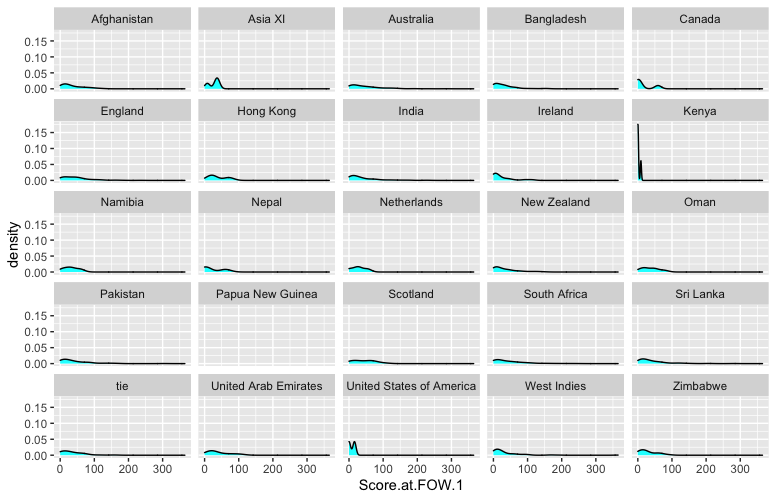
\includegraphics[scale=0.3]{figures/fow1density.png}
        \caption{Density of all teams for first wicket falling}
        \label{alldens1fow}
    \end{minipage}
    \begin{minipage}{0.4\textwidth}
        \centering
        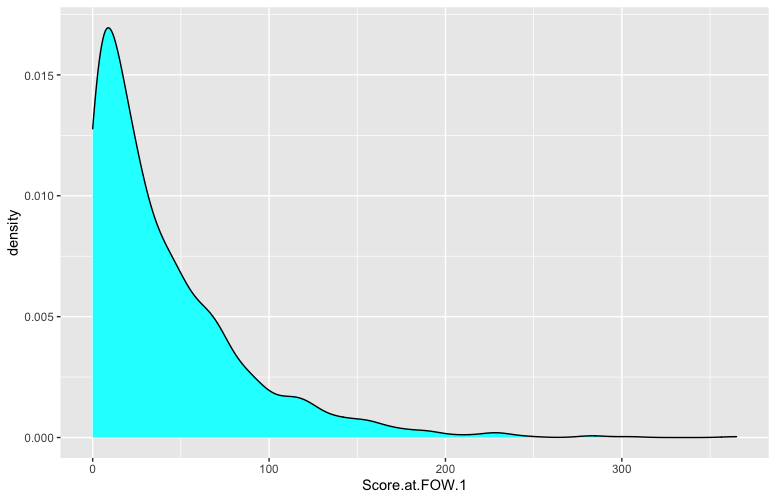
\includegraphics[scale=0.3]{figures/fow1densFull.png}
        \caption{Overall density plot for FOW 1}
        \label{ovrdens1fow}
    \end{minipage}
\end{figure}

\begin{figure}[h]
    \centering
    \begin{minipage}{0.4\textwidth}
        \centering
        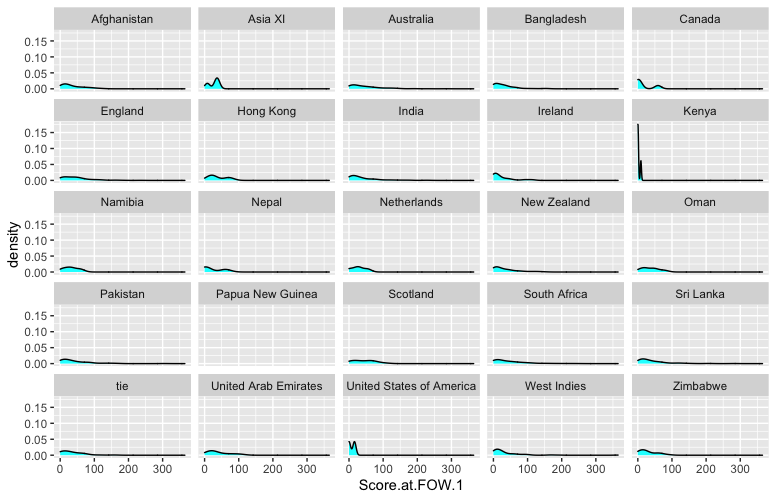
\includegraphics[scale=0.3]{figures/fow1density.png}
        \caption{Density of all teams for fith wicket falling}
        \label{alldens5fow}
    \end{minipage}
    \begin{minipage}{0.4\textwidth}
        \centering
        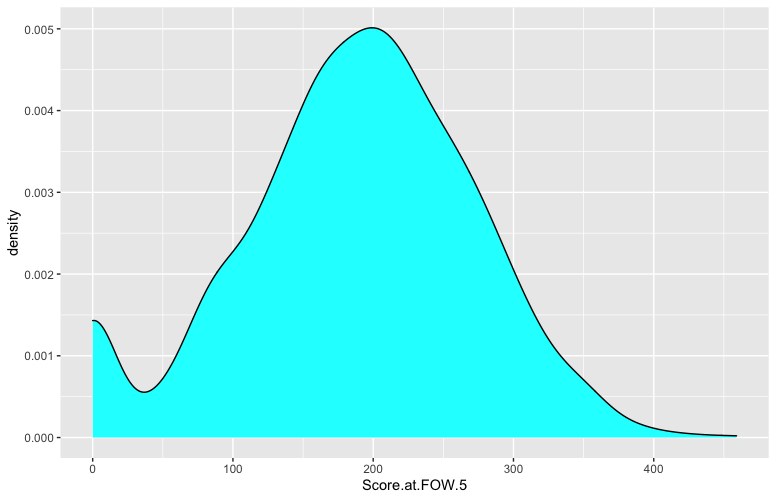
\includegraphics[scale=0.3]{figures/fow5densFull.png}
        \caption{Overall density plot for FOW 5}
        \label{ovrdens5fow}
    \end{minipage}
\end{figure}

\begin{figure}[h]
    \centering
    \begin{minipage}{0.4\textwidth}
        \centering
        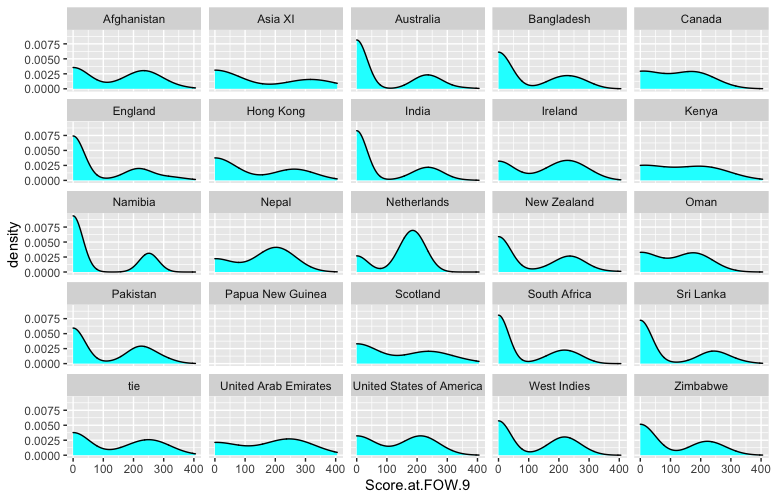
\includegraphics[scale=0.3]{figures/fow9density.png}
        \caption{Density of all teams for ninth wicket falling}
        \label{alldens9fow}
    \end{minipage}
    \begin{minipage}{0.4\textwidth}
        \centering
        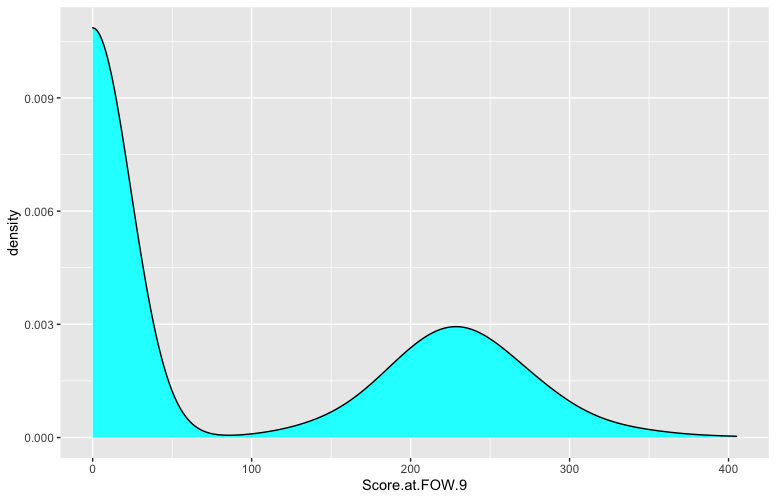
\includegraphics[scale=0.3]{figures/fow9densfull.png}
        \caption{Overall density plot for FOW 9}
        \label{ovrdens9fow}
    \end{minipage}
\end{figure}

In \ref{ovrdens1fow}, we see the density is heavily skewed to the left. This makes sense, as the bowling team will presumably be starting 
their innings by using their best bowlers, who will be hunting to get wickets early on. In \ref{ovrdens5fow}, we see a much more normally distributed
density function. But in actual fact, we see this interesting second, smaller peak appearing lower down in the score. Does this make sense? It's certainly 
not suprising. What these two peaks exemplify is the fact games can go heavily in favour of the bowling team, which can be seen in the first small peak,
wherein they have taken a lot of wickets in quick succession, meaning the later order batters are coming in earlier than usual. Secondly, it shows when the 
batting team is having a good day, because we have this much larger peak around the 200 runs mark.\\

Finally, in \ref{ovrdens9fow}, we can see that the earlier bowling advantage peak is much higer, because the lower order batters are traditionally less skilled 
at batting, and so the bowling team have a distinct advantage in taking wickets against these players. But we also see the second, batting-favoured peak is no much lower.
This corresponds to the scenario in which the earlier batters have laid a good foundation of the game, and the lower-order batters have not had to contribute much to the score.

\section{Outliers in Runs Data}
\label{mse}
In the next chapter, it will be necessary to choose a loss function for improving the neural network that we create. To aid in determining this, we need to look at the
spread of runs scored in a full innings of data. This can be seen in \ref{runsbox}.

\begin{figure}[h]
    \centering
    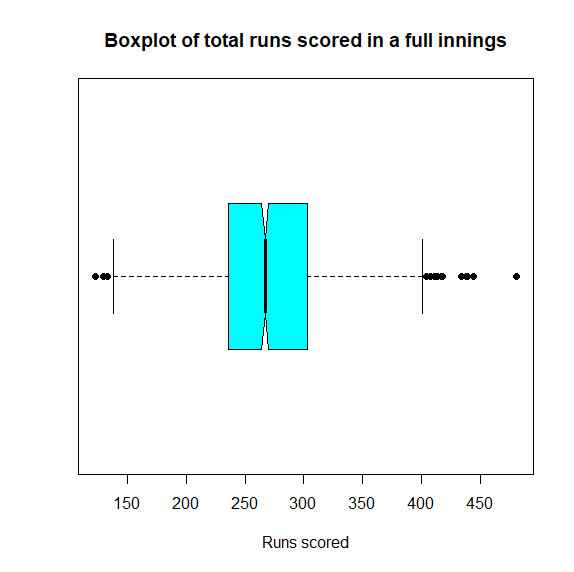
\includegraphics[scale=0.5]{figures/runsbox.png}
    \caption{Boxplot showing the spread of runs scored}
    \label{runsbox}
\end{figure}

There are 363 data points greater than the third quartile, while 671 are below the first quartile. So $25.3\%$ of our data lies above the third quartile, and
$46.7\%$ below the first. For that reason, we make the decision to use the Mean-Squared-Error (MSE) loss function, which is commonplace in regression problems.

\section{On the Normality of Run Totals}
It will be useful in later parts of this dissertation to know whether or not scores are normally distributed. To test whether or not 
they are, we use a Q-Q plot to check. This is a graphical way for checking normality, by comparing the quantiles of a dataset (in this case, scores) to quantiles
drawn from a theoretical distribution. If the resulting points follow a straight line, it is likely that the data came from the distribution.
In this case, we use the R function \textit{qqnorm()} to test if the runs from the 1436 games of a full 50 overs follow a normal distribution.

\begin{figure}[h]
    \label{qqplot}
    \centering
    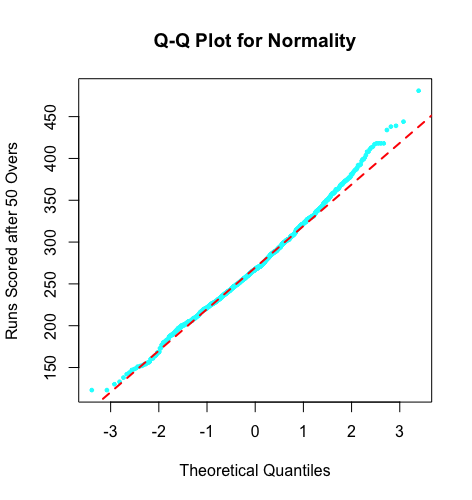
\includegraphics[scale=0.55]{figures/qqnormplot.png}
    \caption{Q-Q plot for runs scored after 50 overs.}
\end{figure}

We can see from the above figure that the plot follows along the straight line and so we can conclude that the scores are infact normally distributed. 
Further, we can calculate the parameters of this distribution using the R functions \textit{mean()} and \textit{var()}. Doing so gives that the distribution
of scores in 50 overs, $S_{50}$, can be given as $S_{50} \sim \mathcal{N}(270.56,51.34^2)$. \\ 

To further test that this is indeed the case, we can create a sample plot based on this distribution, which can be seen in figure \ref{samplenorm}

\begin{figure}
    \label{samplenorm}
    \centering
    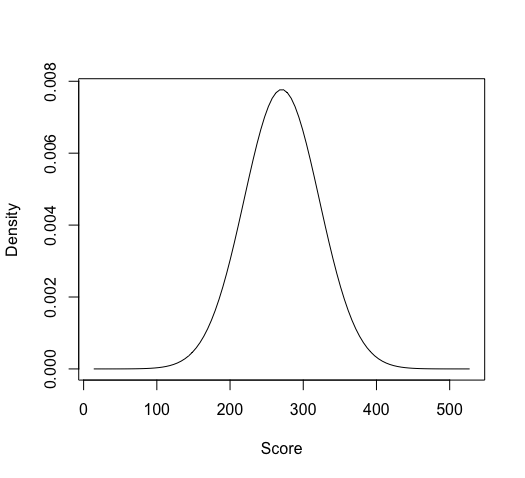
\includegraphics[scale=0.5]{figures/samplenorm.png}
    \caption{Sample plot created from the derived distribution of $S_{50}$}
\end{figure}

With this in mind, we can now look at a density plot for the actual data. This is giving in figure \ref{runsdens}.

\begin{figure}
    \label{runsdens}
    \centering
    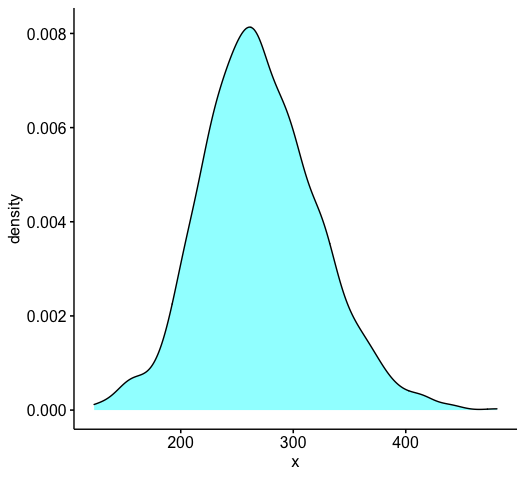
\includegraphics[scale=0.45]{figures/runsdensity.png}
    \caption{Actual density for the runs scored}
\end{figure}

It is unsuprising that runs are normally distributed, but to be able to draw a mean and variance from this will be very helpful in future aspects of the project.

We have seen that first innings scores in a full 50 overs are normally distributed. We can check, using the same methods if runs in a first innings that 
doesn't necessarily go for the full allowance of overs is normally distributed. 

\begin{figure}[h]
    \label{firstInnsQQ}
    \centering
    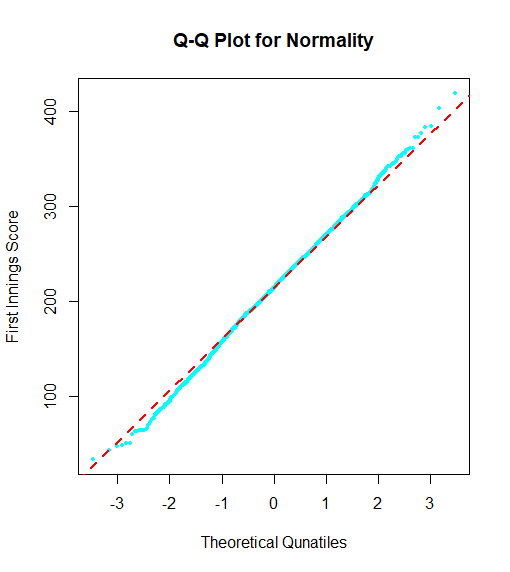
\includegraphics[scale=0.6]{figures/firstInnsQQ.png}
    \caption{Q-Q plt for first innings of varying length}
\end{figure}

We find that $S_{FI} \sim \mathcal{N}(213.49,56.91^2)$. 